In questo capitolo verrà discusso dell'algoritmo C.U.T.E e
del contributo apportato da questo nuovo approccio nell'ambito del \textit{clustering} dei dati di traiettoria.

In primo luogo verrà definito il problema del \textit{Colossal Trajectory Mining},
successivamente saranno presentate l'idea e la realizzazione dell'algoritmo C.U.T.E,
infine saranno formulate alcune considerazione sui punti di forza e limiti di questo nuovo approccio.


\section{Idea generale}\label{sec:cute:idea}
\textit{Cu.Te}, o ClUstering TrajectoriEs, è un algoritmo di clustering overlapping il cui obbiettivo è l'analisi
di gruppi di oggetti in movimento. Questa ricerca viene condotta considerando sia la dimensione spazio-temporale
delle traiettorie sia eventuali dimensioni semantiche (come ad esempio, le municipalità di una città).

Lo scenario reale per la realizzazione di questo algoritmo è stata l'analisi condotta su
un insieme di traiettorie generate a Milano. All'interno di questo studio, i pattern di movimento sono
stati analizzati a diversi livelli.
Una prima analisi è stata condotta dividendo la superfice della città in piccole celle:questa ricerca
ha rivelato i pattern di movimento del traffico, individuando quali potessero essere le strade
maggiormente frequentate.
Succesivamente è stato realizzato uno studio basato sul vicinato: questo ha individuato i flussi di spostamento per specifiche categorie di utenti.
Infine una ricerca basata sulle municipalità ha mostrato quali fossero le aree della città più visitate da differenti gruppi di individui.

Lo scopo di \textit{Cu.Te} è dunque di estrarre i pattern di movimento che avvengono con una certa soglia di frequenza.

L'algoritmo \textit{Cu.Te} è etichettabile come algoritmo di \textit{colossal trajectory mining}.
L'idea alla base del \textit{colossal trajectory mining},
o mining di traiettorie su larga scala, interseca entrambi gli ambiti del clustering di traiettorie
e del colossal itemset mining (~\cref{subsec:problem:cim}).
La prospettiva del mining di itemset ad alta dimensionalità può essere impiegata anche nell'analisi di dati di traiettoria. Considerando la superfice
spazio-temporale coperta dall'insieme delle traiettorie e il numero di queste ultime, nella maggior parte dei casi risulterà evidente
che la dimensionalità di quest'ultimo dato sarà maggiore del precedente.
Risulta quindi possibile applicare algoritmi di mining di itemset su larga scala a dati di traiettoria.
In letteratura è possibile trovare riferimenti ad algoritmi di \textit{colossal itemset mining}~\cite{DBLP:journals/bdr/ApilettiBCGPM17, DBLP:conf/kdd/PanCTYZ03}
, tuttavia nessuno di questi è adatto alla ricerca di pattern di movimento, anche per la mancanza di
criteri di pruning basati sulle dimensioni spazio-temporali. Nonostante quindi la letteratura non
presenti una soluzione adatta, le idee alla base del \textit{colossal itemset mining} risultano sicuramente interessanti.

Parlando poi di clustering di traiettorie, rispetto a quanto trattato nella nella~\cref{sec:problem:trajectoryclustering}, è possibile aggiungere un'ulteriore divisione:
si definisce il clustering partizionante se ogni punto appartiene a un solo cluster, sovrapposto in caso contrario.
Applicando questo principio di classificazione agli algoritmi basati su traiettorie, gli algoritmi partizionanti considereranno la traiettoria nella sua interezza,
assegnandola quindi ad un solo cluster. Questa tipologia di clustering comporta però la perdita di informazioni tra i diversi cluster:
nonostante una traiettoria sia raggruppata in un cluster che massimizza la similarità tra i propri elementi,
questa può comunque condividere pattern interessanti con altre traiettorie appartenenti a cluster differenti.

Per superare il problema descritto sopra, gli algoritmi di clustering sovrapposto effettuano una divisione di ogni traiettoria
in sotto-traiettorie e effettuano un clustering partizionante su queste sotto-traiettorie.
Questa soluzione permette di conservare le relazioni intra-cluster, tuttavia una frammentazione troppo fine può causare
la perdita di \textit{rare pattern}, ad esempio eventi significanti che accadono con una bassa frequenza~\cite{DBLP:journals/tkdd/KohR16, DBLP:journals/geoinformatica/HuangPX06}.

Come già detto nella~\cref{sec:problem:trajectoryclustering}, il clustering classico non esprime vincoli temporali o ulteriori parametri adatti alla ricerca di traiettorie.
Per aggiungere la possibilità di esprimere vincoli sul tempo, sono stati introdotto i \textit{co-movement} patterns descritti nella~\cref{sec:problem:comovements-pattern}; algoritmi come \textit{G.C.M.P},
(~\cref{chapter:chapter2}), \textit{GeT Move}~\cite{DBLP:journals/ijitdm/PhanPT16} e  implementa la ricerca di questi pattern mischiando l'approccio basato su \textit{frequent itemset mining} e il clustering.
Entrambi questi framework discretizzano il tempo in bucket di dimensione finita, su cui poi applicano un clustering basato sulla densità, infine
ricercano pattern di movimento fondendo i vari cluster ottenuti nei differenti istanti temporali.

Rispetto a quanto presentato fin d'ora, \textit{Cu.Te} presenta le seguenti caratteristiche:

\begin{itemize}

  \item Flessibilità nell'impiego di dimensioni: all'interno di \textit{Cu.Te} è possibile aggiungere
  dimensioni personalizzate su cui condurre la ricerca, ad esempio si può espandere la dimensione spazio
  temporale aggiunendo il concetto di municipalità.
  Inoltre sono supportate dimensioni non esclusivamente monotone, come ad esempio i giorni della settimana.

  \item Continuità nello spazio tempo: nella ricerca di \textit{comomvement pattern} è possibile specificare vincoli di contiuità non solo sul tempo, ma anche sullo spazio.

  \item Efficienza nel pruning spazio-temporale: la strategia di pruning impiegata permette di ridurre
  lo spazio di ricerca dell'algoritmo sulla base della natura spazio-temporale delle traiettorie.

  \item Efficacia rispetto a problemi reali: \textit{Cu.Te} mette a disposizione una soluzione distribuita per il problema del \textit{Colossal Trajectory Mining}
  compatibile con dataset costruiti su problemi del mondo reale.
\end{itemize}


L'algoritmo segue tre step per la formazione dei cluster, come anche rappresentato in~\cref{fig:chap-3:cute-overview}

  \begin{figure}
    \centering
    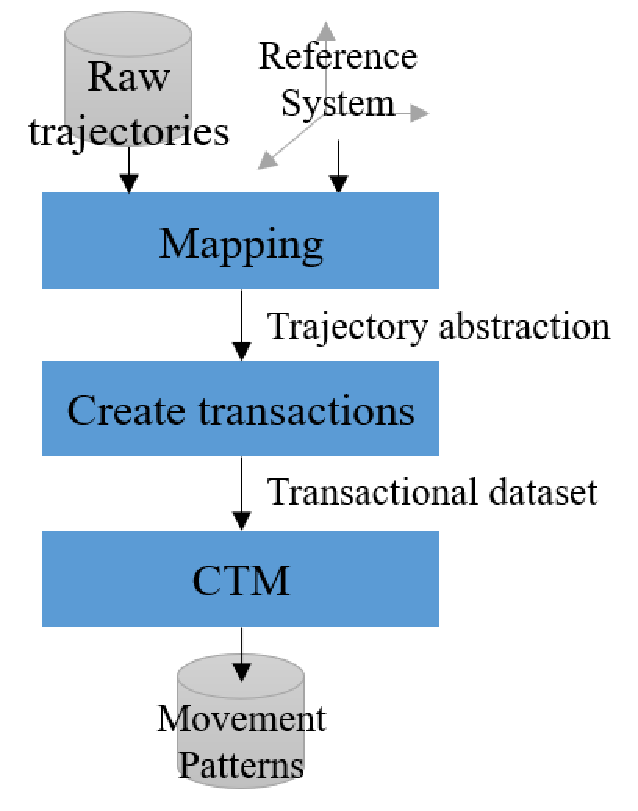
\includegraphics{/sec-3/cute-algorithm-overview.pdf}
    \caption{Rappresentazione grafica delle tre fasi dell'algoritmo Cu.Te,Fonte:~\url{https://which.souce?}}%
    \label{fig:chap-3:cute-overview}
  \end{figure}

  \begin{enumerate}
    \item \textbf{Mapping delle traiettorie:}

    In questo primo passo vengono analizzate le traiettorie presenti nel dataset. Da queste viene determinata la regione spazio-temporale
    in cui tutti gli oggetti si sono mossi. Successivamente l'area di movimento viene divisa in un insieme di celle omogenee per dimensioni nello spazio e nel tempo.
    A questo punto ad ogni traiettoria viene assegnato un insieme di celle secondo il seguente principio: una cella è attribuita ad una traiettoria quando quest'ultima ha
    almeno un punto che ricade entro i confini spazio-temporali della cella.

    \item  \textbf{Creazione delle transazioni:}

    Durante questa fase vengono poste le basi per l'\textit{itemset mining}: scopo di questa parte dell'algoritmo
    è infatti andare a generare l'insieme delle transazioni su cui verrà eseguita la ricerca di pattern.
    Ciò avviene considerando l'ouput della fase precedente e ribaltando la relazione cella traiettoria:
    mentre prima le traiettorie venivano condiderate in termini di celle percorse, ora si considera ogni cella in relazione alle traiettorie che almeno per
    un istante transitano al suo interno.

    \item \textbf{Colossal Trajectory Mining:}

    Ultima e più importante passaggio dell'algoritmo, produce in uscita i pattern di movimento.
    Dato l'output della fase precedente, ovvero un insieme di transazioni appositamemte creato,
    esegue una ricerca di itemset su dati ad alta dimensionalità.

  \end{enumerate}







\subsection{Definizione del problema}\label{subsec:cute:parameters}
Prima di concentrarsi sui singoli passi di \textit{Cu.Te}, occorre definire la formulazione dell'algoritmo.
Innanzitutto si pone necessario riprendere i concetti di itemset, supporto e transazione descritti nella~\cref{sec:problem:frequent-itemset-mining}
e di traiettoria grezza e astrazione di traiettoria presentati nella~\cref{subsec:problem:trajectorydata}.

A queste definizioni va aggiunto il concetto di sistema di riferimento: si definisce un sistema di riferimento un insieme di
quanti completo e continuo all'interno di una regione spazio-temporale.
I sistemi di riferimento sono fondamentali nel determinare le dimensioni spazio-temporali dei punti delle varie traiettorie,
un esempio su tutti può essere una scala di riferimento espressa in coordinate polari.
Tuttavia è possibile definire anche sistemi di riferimento che utilizzano metriche diverse dalle coordinate sopracitate,
ottenendo così diversi effetti sulla rappresentazione dei dati.

Per quanto riguarda invece l'aspetto collegato alla ricerca di itemset,
in \textit{Cu.Te} viene introdotto il concetto di \textit{Cohesion} o coesione: dato un itemset \textit{I} = \{ \textit{i\textsubscript{1}},\ldots, \textit{i\textsubscript{n}}\}
avente supporto definito come \textit{s}, si definisca la funzione \textit{allTransaction(i)} %chktex 36
 che dato un item \textit{i} restituisce l'insieme delle
transazioni che lo supportano. A questo punto è possibile definire la coesione con la seguente formulazione:

\[ coh(I) = \frac{\lvert \lvert allTransaction(\textit{i\textsubscript{1}})~\cap ,\ldots, \cap~allTransaction(\textit{i\textsubscript{n}}) \rvert\rvert}{\lvert \lvert allTransaction(\textit{i\textsubscript{1}})~\cup ,\ldots, \cup~allTransaction(\textit{i\textsubscript{n}}) \rvert\rvert} \]

Considerando che il numeratore corrisponde esattamente a \textit{s}, allora è possibile esprimere l'equazione come:

\[ coh(I) = \frac{s}{\lvert \lvert allTransaction(\textit{i\textsubscript{1}})~\cup ,\ldots, \cup~allTransaction(\textit{i\textsubscript{n}}) \rvert\rvert} \]

La nuova misura permette di misurare la compattezza di un itemset rispetto agli elementi che lo compongono.
La coesione si pone quindi come meccanica di filtraggio aggiuntiva al supporto:
mentre quest'ultimo è una misura in termini assoluti di frequenza, la coesione risulta una metrica relativa alla frequenza dei singoli elementi.
Ne segue che un alto valore di coesione andrà a scartare quegli itemset i cui item risultano molto sparsi all'interno delle transazioni,
mantenendo invece quelli che risultano più compatti.

Una volta definiti questi due concetti, è opportuno elencare e definire i parametri
utilizzati da \textit{Cu.Te}.

\begin{itemize}

  \item Quanto spaziale \textit{s}:
  Definisce la dimemsione spaziale del sistema di riferimento, in relazione alle coordinate polari di ogni punto.

  \item Quanto temporale \textit{t}:
  Definisce la dimensione temporale del sistema di riferimento rispetto al tempo misurato in secondi di ogni punto di una traiettoria.
  \item Soglia di distanza spaziale\(~\epsilon \):
  Dati due punti \textit{p\textsubscript{1}, p\textsubscript{2}} e una funzione di distanza spaziale \textit{d\textsubscript{s}},
  si definisce \(~\epsilon \) come la soglia sotto la quale due punti si considerano vicini.
  \item Soglia di distanza temporale\(~\tau \): analogamente a quanto detto sopra, il parametro \(~\tau \) permette di specificare
  una soglia massima per la distanza tra due punti nel tempo.
  \item Dimensione minima\(~\gamma \): Questo parametro riguarda il numero minimo di item all'interno di ogni itemset restituito in output alla fine dell'algoritmo.
  \item Supporto minimo\(~\alpha \): La frequenza minima oltre cui ogni itemset deve apparire all'interno dell'insieme delle transazioni.
  \item Coesione minima\(~\beta \): Come definito sopra, esprime un limite inferiore alla coesione degli itemset prodotti dall'algoritmo.

\end{itemize}

Grazie a questi parametri, risulta possibile per \textit{Cu.Te} affrontare il problema
della ricerca di \textit{comovement-pattern}, descritto nella \cref{sec:problem:comovements-pattern}.
Scendendo nel dettaglio, \(~\gamma \) esprime la dimensione minima di un gruppo considerato interessante, mentre
\(~\alpha \) il numero minimo di istanti spazio-temporali in cui tutti i membri del gruppo sono considerati vicini.
\(~\epsilon \) rappresenta il criterio di vicinanza spaziale tra due punti, \(~\tau \) invece permette la ricerca dei diversi pattern di movimento:
con \(~\tau \) = 1 si ha un vincolo stringente sulla continuità temporale, andando quindi a ricercare pattern \textit{flock},
dall'altra parte con un valore uguale a \(~\infty \), si rilassa al massimo la continuità temporale, ottenendo
così dei risultati classificabili come \textit{Swarm}. Infine con qualunque valore intermedio tra 1 e  \(~\infty \),
\textit{Cu.Te} esegue la ricerca di pattern \textit{Group} degeneri, ovvero con vincolo \textit{L} posto uguale a 1.




\subsection{Mapping del dataset}\label{subsec:cute:mappingdataset}
Inizialmente, il dataset delle traiettorie è composto da un insieme di punti aventi le seguenti caratteristiche:
una dimensione temporale espressa in secondi, due coordinate spaziali per determinare la sua posizione rispetto a un sistema di coordinate polari e
infine un identificatore di traiettoria. A queste dimensioni possono essere poi aggiunte altre informazioni, che non sono prese in considerazione durante l'esecuzione dell'algoritmo.

Scopo di questa prima fase di \textit{Cu.Te} è determinare un sistema di riferimento per i punti all'interno del dataset ed esprimere questi ultimi in
relazione al nuovo sistema.

Come indicato nella~\cref{subsec:cute:parameters}, è possibile determinare un sistema di riferimento che più aderisce alle esigenze del problema.
In questo caso la necessità principale in vista della fase di \textit{Colossal Trajectory Mining} è la ridotta dimensionalità dello spazio-tempo rispetto al numero di traiettorie
processate: si rende infatti necessario avere un numero di riferimenti spazio-temporali strettamente inferiorie alle traiettorie presenti nel database.

L'idea per risolvere questa esigenza è la divisione della superficie spazio-temporale in celle omogenee per range. Dato l'intero volume dello spazio-tempo
coperto dalle traiettorie nel dataset, questo viene partizionato in parallelepipedi di medesime dimensioni. Una cella \textit{c} è un parallepipedo, generato dal
partizionamento dello spazio-tempo coperto dalle traiettorie, avente un indice univoco.
Questa suddivisione costituisce quindi il nuovo sistema di riferimento del problema, è necessario quindi esprimere i punti all'interno del dataset rispetto a questo nuovo sistema.

Partendo dallo spazio, ogni punto di traiettoria, per definizione, determina la propria posizione sulla superficie terrestre utilizzando due coordinate, latitudine e longitudine.
Prendendo in considerazione l'area di un insieme di traiettorie, il processo per la generazione di celle spaziali è il seguente: per prima cosa si determina, mediante
il parametro \textit{s} la dimensione dei lati spaziali di una cella; successivamente si definisce la funzione \textit{pointToCell}, tale funzione ha il compito
di restituire, dato un punto, la cella di appartenenza. La cella in questione viene calcolata supponendo di scomporre la superficie terrestre in quadrati aventi lato \textit{s}
a partire da Null Island (punto avente latitudine e longituidne pari a zero)~\footnote{\url{https://blogs.loc.gov/maps/2016/04/the-geographical-oddity-of-null-island/}}.
In~\cref{fig:chap-3:milan-cell-division} è possibile vedere un esempio di divisione in celle applicato sulla città di Milano.

\begin{figure}
  \centering
  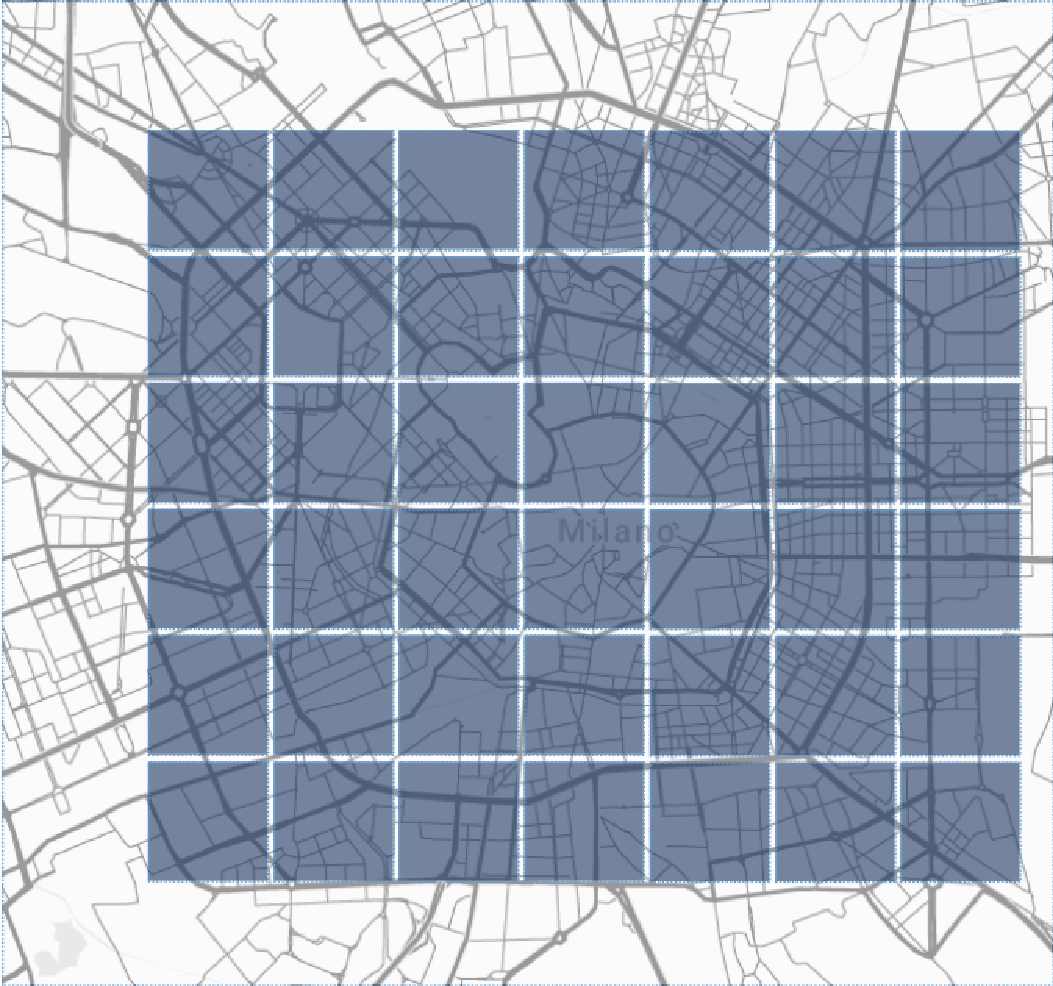
\includegraphics[scale=.6]{/sec-3/MilanCells.pdf}
  \caption{Suddivisione della città di Milano in celle,Fonte:~\url{https://which.souce?}}%
  \label{fig:chap-3:milan-cell-division}
\end{figure}

Per quanto riguarda la dimensione temporale invece, le possibilità a disposizione sono diverse, ma tra tutte si è scelto di supportare due principali scale: una basata sulle ore del giorno mentre l'altra sui giorni della settimana.
Rispetto a una metrica di tempo monotona basata su data e ora di ogni singolo punto, come ad esempio in \textit{G.C.M.P}, una scala circolare ha due vantaggi: il primo riguarda
il supporto a pattern ciclici che verrebbbero ignorati da una metrica monotona e in secondo luogo il ridotto range di valori della scala (da 0 a 23 in caso di scala giornaliera, da 0 a 6 in quella settimanale)
previene l'esplosione nel numero di celle al crescere del dataset.

Una volta determinata il lato spaziale delle celle e la durata temporale, processando le traiettorie nel dataset mediante una variazione della funzione \textit{pointToCell} adattata alla
gestione di celle tridimensionali, viene generato l'insieme delle celle \textit{C}. Questo set contiene tutte le celle, determinate dall'apposita funzione, tali che almeno
un punto di una traiettoria appartiene a quella cella. Questo approccio alla generazione delle celle garantisce che non vengano generate celle vuote, ovvero dove non passa nessuna traiettoria,
garantendo quindi una maggiore efficenza rispetto alla suddivisione assoluta della superficie spazio-temporale coperta dal dataset.

Ottenuto l'insieme delle celle, è necessario per concludere questa prima fase esprimere ogni traiettoria nel nuovo sistema di riferimento: così facendo una traiettoria non sarà più definita come
la composizione di diversi punti isolati nel tempo, ma come un'insieme di celle. La~\cref{fig:chap-3:trajectory-cell-division} mostra un esempio di conversione in un sistema di riferimento basato su celle:

\begin{figure}
  \centering
  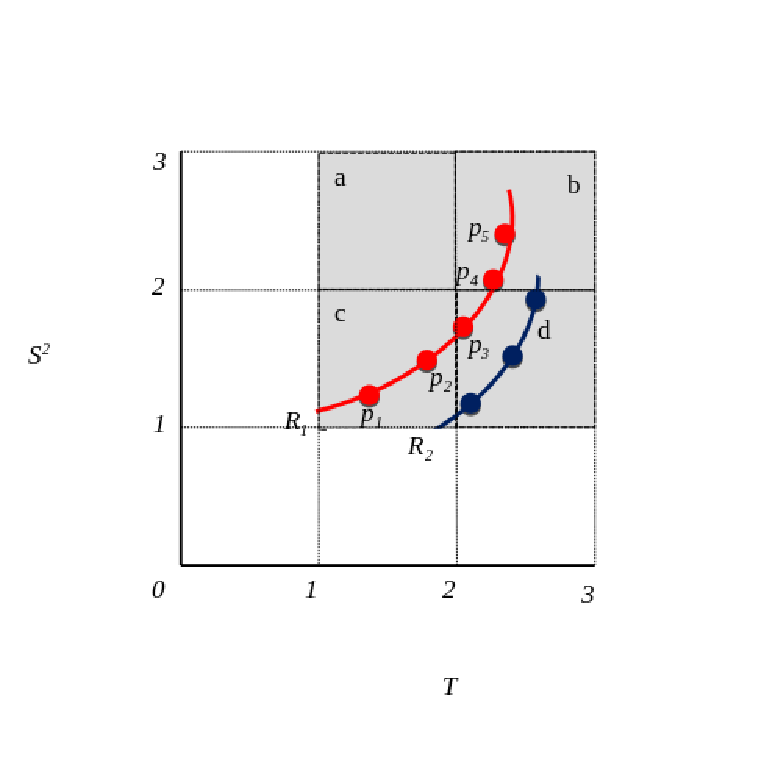
\includegraphics[scale=.8]{/sec-3/TrajectoryCellDecomposition.pdf}
  \caption{Mapping di due traiettorie, \textit{R\textsubscript{1}, R\textsubscript{2}} in un sistema di riferimento basato su celle.}%
  \label{fig:chap-3:trajectory-cell-division}
\end{figure}

Prendendo in considerazione le traiettorie \textit{R\textsubscript{1}, R\textsubscript{2}}, è possibile vedere come i punti \textit{p\textsubscript{1}, p\textsubscript{2}} appartengano alla cella \textit{c},
\textit{p\textsubscript{3}} a \textit{d} mentre \textit{p\textsubscript{4}, p\textsubscript{5}} a \textit{b}; analogamente ogni punto della traiettoria \textit{R\textsubscript{2}} sia attribuibile a \textit{d}.
Il set di celle del problema sarà quindi composto dalle seguenti celle: \textit{\textless b, c, d \textgreater} mentre le due traiettore saranno espresse in funzione del nuovo sistema di rifermimento come segue:

\begin{itemize}

  \item \textit{R\textsubscript{1}}: \{ \textit{b,c,d} \}
  \item \textit{R\textsubscript{2}}: \{ \textit{d} \}

\end{itemize}

Va sottolineato infine che, sebbene appaia nell'immagine, la cella \textit{a} non viene effettivamente generata, poiché nessuna traiettoria ha un punto entro i suoi confini.

Una volta che le traiettorie sono state espresse nelle nuove coordinate, questo primo passo dell'algoritmo giunge a termine.

Nonostante le operazioni eseguite in questa fase possano sembrare lineari, le basi che vengono gettate influenzano l'esecuzione dell'algoritmo e gli stessi risultati finali:
tra tutte, la scelta delle dimensioni di ogni cella influenza molto i passaggi successivi. Celle piccole produrranno traiettorie lunghe, estendendo il possibile spazio di ricerca di ogni cluster.
Tanto più amplio lo spazio di ricerca, tanto più a lungo dura la sua esplorazione, tuttavia è possibile eseguire una ricerca più fine su di esso.
Lati spaziali più ampli e dimensioni temporali ridotte generano celle più grandi, con uno spazio di ricerca più ridotto e risultati più grezzi.

Nonostante quanto affermato all'inizio, non è completamente corretto dire che tutti i dati che non siano collegati alla posizione nello spazio-tempo della traiettoria siano ignorati.
È infatti possibile considerare un numero variabile di dimensioni durante il processo di generazione delle celle. Tale aggiunta infatti non fa altro che andare ad aumentare la dimensionalità della singola cella,
ciò implica un numero maggiore di celle in cui dover convertire una traiettoria, ma il risultato finale della fase sarà il medesimo, l'unica differenza sarà nell'avere mediamente traiettorie
associate a un numero maggiore di celle.



\subsection{Creazione delle transazioni}\label{subsec:cute:transactioncreation}
Nella prima fase viene prodotto un dataset nella forma \textit{<t\textsubscript{i}, (c\textsubscript{1},\ldots,c\textsubscript{n})>},
dove \textit{t\textsubscript{i}} rappresenta l'id di una certa traiettoria, mentre \textit{c\textsubscript{1},\ldots,c\textsubscript{n}}
l'insieme di celle in cui tale percorso è stato convertito.
Questo dataset tuttavia non è ancora adatto ad essere sottoposto a mining, poiché in questa situazione l'insieme delle transazioni è composto dalle traiettorie,
mentre quello delle feature dalle celle.
Un'operazione di ricerca di regole associative va ad individuare tra le feature quelle che compaiono assieme con almeno una certa frequenza,
quindi in questo caso il risultato dell'algoritmo sarebbe varii raggruppamenti di celle.
Questi insiemi possono essere sicuramente utili ad individuare percorsi frequenti e trafficati, ma non sono in grado di descrivere gruppi di movimenti comuni ad un certo insieme di oggetti.

Scopo di questo secondo passo di \textit{Cu.te} è quindi modificare il dataset ottenuto dalla prima fase
in modo da renderlo valido per la ricerca di pattern di movimento.
Per realizzare questa trasformazione, occorre invertire il ruolo di celle e traiettorie all'interno del dataset: prendendo come
ipotesi di invertire la relazione tra traiettoria e insieme di celle che la compongono, si ottiene la versione trasposta del dataset originale.
La versione invertita del database sarà quindi composta dalle singole celle del problema che ora saranno identificate
come le transazioni, mentre il ruolo delle traiettorie sarà di feature. Così facendo ad ogni cella sarà associato l'insieme delle traiettorie di cui
fa parte.
In questa situazione la ricerca di itemset frequenti produce raggruppamenti di traiettorie che hanno una frequenza maggiore
a una certa soglia di supporto.
Tale soglia può essere interpretata come il numero minimo di celle, ovvero di istanti spazio-temporali, che
l'intero gruppo di traiettorie deve aver condivisio per essere considerato interessante.
Alla luce di questa interpreatzione, diviene chiaro che questo vincolo svolge la stessa identica funzione del parametro \textit{k} definito nella~\cref{sec:comovements-pattern},
per quanto riguarda invece \textit{m}, questo è espresso con  \(~\gamma \), presentato nella~\cref{subsec:cute:parameters}; infine \textit{g} è espresso come \(~\tau \) nella formalizzazione di \textit{Cu.Te}.

Invertendo il dataset è quindi possibile eseguire una ricerca di comovements pattern, ma l'inversione ha un'altra importante proprietà:
analizzando il rapporto tra il numero di celle generate nella prima fase e di traiettorie in tutto il dataset, è corretto affermare che
la quantità di queste ultime superi di gran lunga l'altra. La ricerca di pattern di movimento in città presenta infatti un'area spazio-temporale
ridotta rispetto agli oggetti che si muovono sopra questa superficie.
Di conseguenza il dataset che considera come transazioni le celle e come feature le traiettorie sarà etichettabile come dataset ad alta dimensionalità, adatto quindi a essere processato con le tecniche proprie del
\textit{Colossal Trajectory Mining}.




\subsection{Colossal Trajectory Mining}\label{subsec:cute:ctm}
Ultimo e più importante passaggio dell'algoritmo: dato il dataset prodotto in output dalla fase precedente,
viene eseguita una ricerca di pattern di co-movimento utilizzando i principi del \textit{Colossal Trajectory Mining}.




\section{Dettagli implementativi}\label{sec:implementation}

\section{Punti di forza e limiti}\label{sec:cute:strenght}


